%%%%%%%%%%%%%%%%%%%%%%%%%%%%%%%%%%%%%%%%%%%%%%%%%%%%%%%%%%%%%%%%%%%%%%%%%%%%%%%%%%%%%%%%%%%%%%%%%%%%%%%%%%%%%%%%%%%%%%%%%%%%%%%%%%%%%%%%%%%%%%%%%%%%%%%%%%%%%%%%%%%
% Written By Michael Brodskiy
% Class: Embedded Design: Enabling Robotics
% Professor: S. Shazli
%%%%%%%%%%%%%%%%%%%%%%%%%%%%%%%%%%%%%%%%%%%%%%%%%%%%%%%%%%%%%%%%%%%%%%%%%%%%%%%%%%%%%%%%%%%%%%%%%%%%%%%%%%%%%%%%%%%%%%%%%%%%%%%%%%%%%%%%%%%%%%%%%%%%%%%%%%%%%%%%%%%

\documentclass[12pt]{article} 
\usepackage{alphalph}
\usepackage[utf8]{inputenc}
\usepackage[russian,english]{babel}
\usepackage{titling}
\usepackage{amsmath}
\usepackage{graphicx}
\usepackage{enumitem}
\usepackage{amssymb}
\usepackage[super]{nth}
\usepackage{everysel}
\usepackage{ragged2e}
\usepackage{geometry}
\usepackage{multicol}
\usepackage{fancyhdr}
\usepackage{cancel}
\usepackage{siunitx}
\usepackage{physics}
\usepackage{lastpage}
\usepackage{tikz}
\usepackage{mathdots}
\usepackage{yhmath}
\usepackage{cancel}
\usepackage{color}
\usepackage{array}
\usepackage{multirow}
\usepackage{gensymb}
\usepackage{tabularx}
\usepackage{extarrows}
\usepackage{booktabs}
\usetikzlibrary{fadings}
\usetikzlibrary{patterns}
\usetikzlibrary{shadows.blur}
\usetikzlibrary{shapes}

\geometry{top=1.0in,bottom=1.0in,left=1.0in,right=1.0in}
\newcommand{\subtitle}[1]{%
  \posttitle{%
    \par\end{center}
    \begin{center}\large#1\end{center}
    \vskip0.5em}%

}
\usepackage{hyperref}
\hypersetup{
colorlinks=true,
linkcolor=blue,
filecolor=magenta,      
urlcolor=blue,
citecolor=blue,
}

\pagestyle{fancy}

\lfoot[\vspace{-15pt} \hline]{\vspace{-15pt} \hline}
\rfoot[\vspace{-15pt} \hline]{\vspace{-15pt} \hline}
\cfoot[\thepage]{\thepage}
\chead[\textsc{Embedded Systems}]{\textsc{Embedded Systems}}
\lhead[\textsc{EECE2160, CRN: 32014}]{\textsc{EECE2160, CRN: 32014}}
\rhead[\textsc{Page \thepage \hspace{1pt} of \pageref{LastPage}}]{\textsc{Page \thepage \hspace{1pt} of \pageref{LastPage}}}



\title{Lab 7 Pre-Lab Submission}
\date{\today}
\author{Michael Brodskiy\\ \small Professor: S. Shazli}

\begin{document}

\maketitle

\begin{figure}[H]
  \centering
  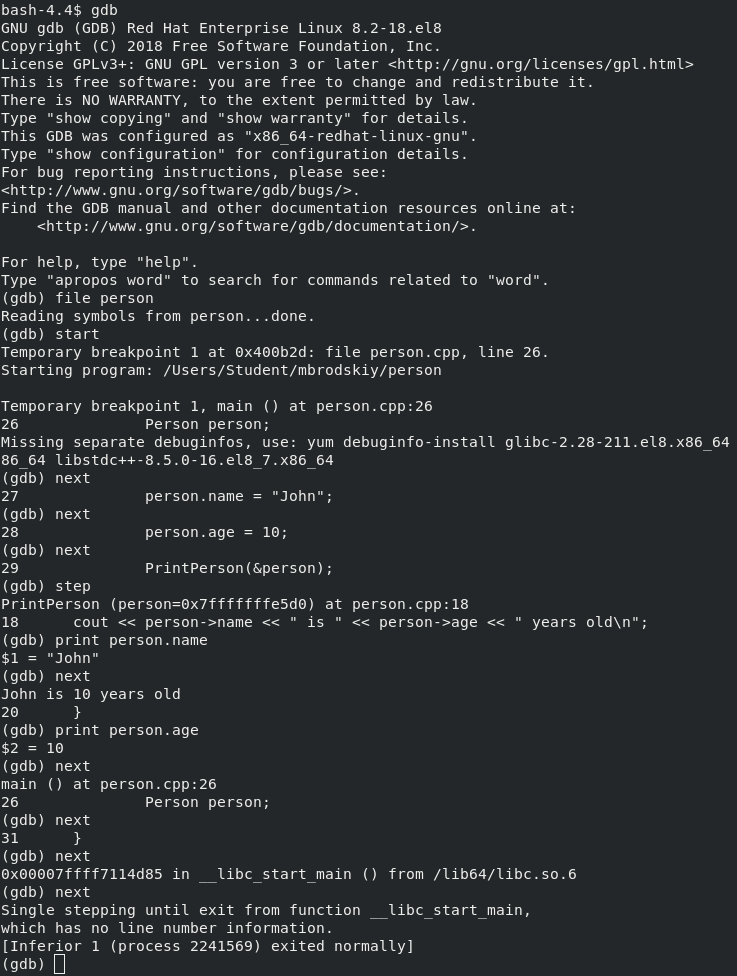
\includegraphics[width=.7\textwidth]{Figures/gdb.png}
  \caption{\texttt{gdb} output}
  \label{fig:1}
\end{figure}

The \texttt{gdb} commands may be explained as follows:

\begin{itemize}

  \item \texttt{file person} selects the binary called person as the file for analysis

  \item \texttt{start} begins analysis of ``person''

  \item \texttt{next} moves to the next point of interest

  \item \texttt{step} enters the function at the current line

  \item \texttt{print} prints the known information for a certain, specified value

\end{itemize}

\lstinputlisting[
    caption=Menu Printing Code, % Caption above the listing
    label=lst:L1, % Label for referencing this listing
    language=C++, % Use C++ functions/syntax highlighting
    frame=single, % Frame around the code listing
    showstringspaces=false, % Don't put marks in string spaces
    numbers=left, % Line numbers on left
    numberstyle=\tiny, % Line numbers styling
    backgroundcolor=\color{black!5}, % Set background color
    keywordstyle=\color{magenta!80}, % Set keyword color
    commentstyle=\color{blue!80}, % Set comment color
    stringstyle=\color{green!80}, % Set string color
    breaklines=true
  ]{Code/PreLab.cpp}

\begin{figure}[H]
  \centering
  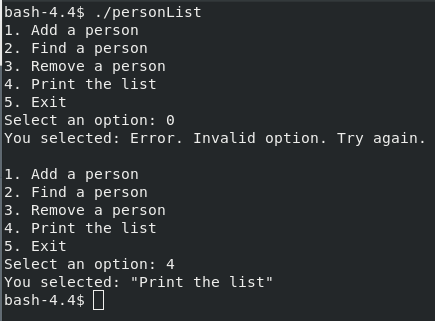
\includegraphics[width=.9\textwidth]{Figures/output.png}
  \caption{Sample menu output}
  \label{fig:2}
\end{figure}

\end{document}

